% By J. Leon, Beerware licence is acceptable...
\documentclass[tikz,border=10pt]{standalone}
%\documentclass[crop,tikz,convert={outext=.svg,command=\unexpanded{pdf2svg \infile\space\outfile}},multi=false]{standalone}

%\usepackage{tikz}
\usetikzlibrary{positioning, fit, arrows.meta, shapes}

\begin{document}

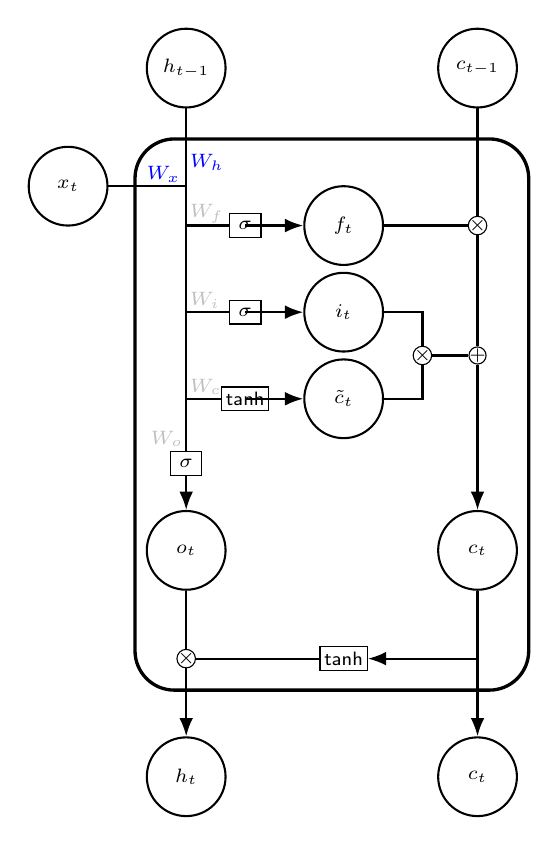
\begin{tikzpicture}[
    % GLOBAL CFG
    font=\sf \scriptsize,
    >=LaTeX,
    % Styles
    cell/.style={% For the main box
        rectangle, 
        rounded corners=5mm, 
        draw,
        very thick,
        },
    operator/.style={%For operators like +  and  x
        circle,
        draw,
        inner sep=-0.5pt,
        minimum height =.2cm,
        },
    function/.style={%For functions
        ellipse,
        draw,
        inner sep=1pt
        },
    ct/.style={% For external inputs and outputs
        circle,
        draw,
        line width = .75pt,
        minimum width=1cm,
        inner sep=1pt,
        },
    gt/.style={% For internal inputs
        rectangle,
        draw,
        minimum width=4mm,
        minimum height=3mm,
        inner sep=1pt
        },
    mylabel/.style={% something new that I have learned
        font=\scriptsize\sffamily
        },
    ArrowC1/.style={% Arrows with rounded corners
        rounded corners=0cm,%.25cm,
        thick,
        },
    ArrowC2/.style={% Arrows with big rounded corners
        rounded corners=0cm,%.5cm,
        thick,
        },
    ]

%Start drawing the thing...    
    % Draw the cell: 
    \node [cell, minimum height =7cm, minimum width=5cm] at (0.35,-0.4){} ;

    \newcommand{\step}{1.1}

    % Draw activation functions
    \node [gt] (sigma_f) at (-0.75,2) {$\sigma$};
    \node [gt] (sigma_i) at (-0.75,2-\step) {$\sigma$};
    \node [gt, minimum width=0.6cm] (tanh_c) at (-0.75,2-2*\step) {tanh};
    \node [gt] (sigma_o) at (-1.5,2-2.75*\step) {$\sigma$};
    
    \node [gt, minimum width=0.6cm] (tanh_end) at (0.5,2-5*\step) {tanh};
    
    
    \node[text width=0.3cm, text = blue] at (-1.85,2.65) {$W_x$};
    \node[text width=0.3cm, text = blue] at (-1.3,2.8) {$W_h$};
    
    
    \node[text width=0.3cm, text=lightgray] at (-1.3,2.15) {$W_f$};
    \node[text width=0.3cm, text=lightgray] at (-1.3,2.15-\step) {$W_i$};
    \node[text width=0.3cm, text=lightgray] at (-1.3,2.15-2*\step) {$W_c$};
    \node[text width=0.3cm, text=lightgray] at (-1.8,2.15-2.6*\step) {$W_o$};
    
    % Draw Internal 
    \node[ct] (ft) at (0.5,2) {$f_t$};
    \node[ct] (it) at (0.5,2-\step) {$i_t$};
    \node[ct] (hatCt) at (0.5,2-2*\step) {$\tilde{c}_t$};
    \node[ct] (ot) at (-1.5,2-3.75*\step) {$o_t$};

   % Draw multiplication and addition operators
    \node [operator] (mux_conveyor) at (2.2,2) {$\times$};
    \node [operator] (add_conveyor) at (2.2,0.35) {+};
    \node [operator] (mux_i_and_c) at (1.5,0.35) {$\times$};
    \node [operator] (mux_end) at (-1.5,2-5*\step) {$\times$};


    % Draw External inputs? named as basis c,h,x
    %\node[ct, label={[mylabel]Cell}] (c_old) at (2.2,4) {$c_{t-1}$};
    \node[ct] (c_old) at (2.2,4) {$c_{t-1}$};
    \node[ct] (h_old) at (-1.5,4) {$h_{t-1}$};
    \node[ct] (x) at (-3,2.5) {$x_t$};

    % Draw External outputs? named as basis c2,h2,x2
    \node[ct] (c2) at (2.2,2-3.75*\step) {$c_t$};
    \node[ct] (h2) at (-1.5,-5) {$h_t$};
    \node[ct] (c2_final) at (2.2,-5) {$c_t$};
    

% Start connecting all.
    %Intersections and displacements are used. 
    % Drawing arrows    
    \draw [->, ArrowC1] (c_old) -- (mux_conveyor) -- (add_conveyor) -- (c2);

    % Inputs
    \draw [ArrowC1] (x) -| (sigma_o);
    \draw [->, ArrowC1] (h_old) -- (sigma_o) -- (ot);
    \draw [->, ArrowC1] (h_old)++(0,-0.5) |- (sigma_f) |- (ft);
    \draw [->, ArrowC1] (h_old)++(0,-0.5) |- (sigma_i) |- (it);
    \draw [->, ArrowC1] (h_old)++(0,-0.5) |- (tanh_c) |- (hatCt);
    
    % f_t to the conveyor
    \draw [ArrowC1] (ft) -- (mux_conveyor);
    
    % i_t and hatC_t to the conveyor
    \draw [ArrowC1] (it) -| (mux_i_and_c)++(0,-0.5);
    \draw [ArrowC1] (hatCt) -| (mux_i_and_c)++(0,-0.5);
    \draw [ArrowC1] (mux_i_and_c) -- (add_conveyor);
    
    % end
    \draw [->, ArrowC1] (c2) |- (tanh_end);
    \draw [ArrowC1] (tanh_end) -- (mux_end);
    \draw [ArrowC1] (ot) -- (mux_end);
    \draw [->, ArrowC1] (mux_end) -- (h2);
    \draw [->, ArrowC1] (c2) -- (c2_final);
    
    %\draw [ArrowC1] (x) -- (x -| sigma_o)-| (sigma_f);
    %
    %\draw [ArrowC2] (h_old)++(0,-2) -- (sigma_f); % -- (mux_conveyor); 
    %\draw [ArrowC1] (h_old -| sigma_i)++(0,0.5) -| (sigma_i);
    %\draw [ArrowC1] (h_old -| tanh_c)++(0,0.5) -| (tanh_c);
    %\draw [ArrowC1] (x) -- (x |- h_old)-| (tanh_c);

    % Internal
%    \draw [->, ArrowC2] (sigma_f) -- (mux_conveyor);
%    \draw [->, ArrowC2] (sigma_i) |- (mux_i_and_c);
%    \draw [->, ArrowC2] (tanh_c) -- (mux_i_and_c);
%    \draw [->, ArrowC2] (sigma_o) |- (mux_end);
%    \draw [->, ArrowC2] (mux_i_and_c) -- (add_conveyor);
%    \draw [->, ArrowC1] (add_conveyor -| tanh_end)++(-0.5,0) -| (tanh_end);
%    \draw [->, ArrowC2] (tanh_end) -- (mux_end);

    %Outputs
%    \draw [-, ArrowC2] (mux_end) |- (h2);
%    \draw (c2 -| x2) ++(0,-0.1) coordinate (i1);
%    \draw [-, ArrowC2] (h2 -| x2)++(-0.5,0) -| (i1);
%    \draw [-, ArrowC2] (i1)++(0,0.2) -- (x2);

\end{tikzpicture}
\end{document}